\subsection{\href{https://dl.acm.org/citation.cfm?id=3276490}{OOPSLA2018}: Julia}
\label{paper:oopsla2018Julia}

The Julia programming language aims to decrease the gap between productivity and performance
languages. On one hand, it provides productivity features like dynamic typing, garbage collection,
and multiple dispatch. On the other, it has a type-specializing just-in-time compiler and lets
programmers control the layout of data structure in memory. Julia, therefore, promises scientific
programmers the ease of a productivity language at the speed of a performance language.
Julia语言旨在缩小性能语言(C、C++、Fortran)
和生产力语言(如Python、MATLAB、R)之间的差距。
一方面,它提供像动态定型、垃圾收集、多分派等提高生产力的特性;
另一方面它有类型特化的即时编译器,
并让程序员控制数据结构在内存中的布局。
因此,Julia向科学计算程序员承诺以高性能语言的速度获得高生产力语言的简易性。

The key to performance in Julia lies in the synergy
between language design, implementation techniques and
programming style.
Julia的性能关键在于语言设计、实现技术和编程风格之间的协同作用。

\subsubsection{性能}
\label{paper:oopsla2018Julia:perf}
Fig.\ref{fig:julia:personyear}给出了几种语言实现所花费的人年。
\begin{figure}[htbp]
    \centering
    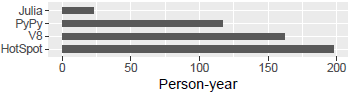
\includegraphics[width=0.5\textwidth]{img/julia-personyear.png}
    \caption{Time spent on implementations}
    \label{fig:julia:personyear}
\end{figure}

为评测语言的相对性能,选择\href{https://benchmarksgame-team.pages.debian.net/benchmarksgame/}{PLBG}中的用
C、JavaScript、Python分别实现的10个小程序,
另外由Julia开发者编写相应的Julia版本。
使用PLBG的方法,测量去除注释和重复的空白符后的代码的最小Gzip压缩包的大小,
Julia的有6KB,JavaScript的有7.4KB, Python有8.3KB, C有14.2KB。
Fig.\ref{fig:julia:slowdown}比较了4种语言相比C语言版本的规范化运行时间。测试使用的相关编译器版本是Julia v0.6.2、CPython 3.5.3、V8/Node.js v8.11.1和GCC 6.3.0 -O2,
评测的机器是Intel i7-950 3.07GHz, 10GB RAM,
操作系统是Debian 9.4。
结果表明,Julia的性能胜过Python和JavaScript(spectralnorm除外);多数程序的Julia版本的运行时间是C版本的2倍以内,
\textbf{性能下降的原因可能是内存操作}(Julia靠垃圾收集器管理内存)。
Julia禁止像C那样显式管理内存,它在堆中分配结构,
栈分配仅用在有限的情况下,不允许指针算术运算。
\begin{figure}[htbp]
    \centering
    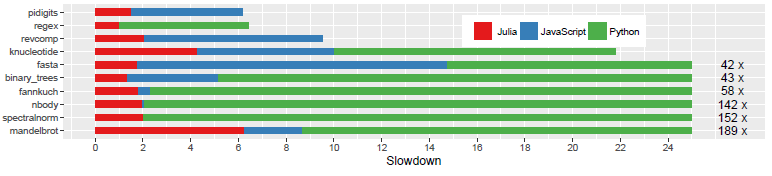
\includegraphics[width=0.9\textwidth]{img/julia-perf.png}
    \caption{Slowdown of Julia, JavaScript, and Python relative to C}
    \label{fig:julia:slowdown}
\end{figure}

\subsubsection{Julia语言}
\label{paper:oopsla2018Julia:lang}
Values
Type Declarations
Type Annotations
Subtyping.
Dynamically-checked Type Assertions.
Multiple Dispatch.
Metaprogramming: Macros, Reflection, Epochs.

Object oriented programming. Julia不支持基于类的面向对象编程风格,缺少封装机制。

Functional programming.
Julia支持高阶函数、immutable-by-default values,
但是没有arrow types.

Gradual typing.

\subsubsection{Julia的实现}
\label{paper:oopsla2018Julia:impl}
\textbf{方法特化}(Method Specialization).
类型推断(Type Inference).
方法内联(Method Inlining).
对象拆箱(Object Unboxing)

